\section{Preliminary Models}
\subsection{Daimler Models}

\subsubsection*{Introduction}

As previously described in D1.2 and the DoW, the basic settings of the DAIMLER's use-case are as follows. Let us suppose we are driving our car, which will be referred as the EGO vehicle, in a highway. This EGO vehicle is equipped with a video camera, radar and some on-board sensors.  Using the data provided by these sensors, the problem consists in the early recognition a maneuver either of the EGO or another relevant car in the traffic scene. In total, the system is expected to recognized the following set of of maneuvers (a visual description of them is given below in Figure \ref{Figure:DaimlerManeuvers}):
\begin{enumerate}

\item \textbf{Object-CutOut}:  A vehicle that was driving in front of us is leaving the EGO lane.
\item \textbf{Object-CutIn}: A vehicle is moving to the lane where the EGO vehicle is placed.
\item \textbf{EGO-CutOut}: The EGO vehicle is leaving the lane where it was driving.
\item \textbf{EGO-CutIn}: The EGO vehicle is moving to a new lane, where there is a vehicle that will be placed behind once the lane change is performed. 
\item \textbf{Object-Follow}: There is no lane change. The EGO is driving and there is some other vehicle in front.
\item \textbf{Lane-Follow}: There is no lane change. The EGO is driving and there is not any other vehicle in front.
\end{enumerate}

\begin{figure}
\begin{center}
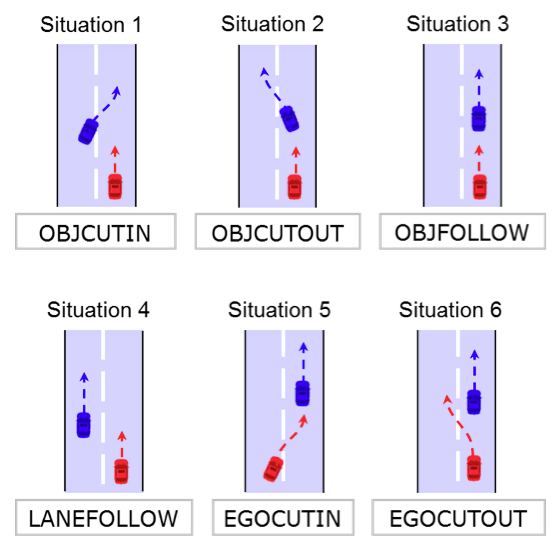
\includegraphics[scale=0.4]{./figures/DaimlerManeuvers}
\caption{\label{Figure:DaimlerManeuvers}Different maneuvers which should be identified by the AMIDST system.  Red blocks represents the EGO vehicle and blue blocks represents other vehicles in the scene. In the first four maneuvers, there is a lane change event or, under Daimler’s terminology, a ``Lane Marking Crossing'' (LMC) event. 
}
\end{center}
\end{figure}

The data used to address this problem do not contain raw data from the video, radar and on-board sensors. The early maneuver recognition system directly works with the so-called ``object data'', which contains ``high level'' representations or features describing the ``traffic scene'' such as EGO’s speed, distance between EGO and another vehicle in front, etc.  Figure \ref{Figure:DaimlerDataFlow} contains a visual description of the current data flow. 

\begin{figure}
\begin{center}
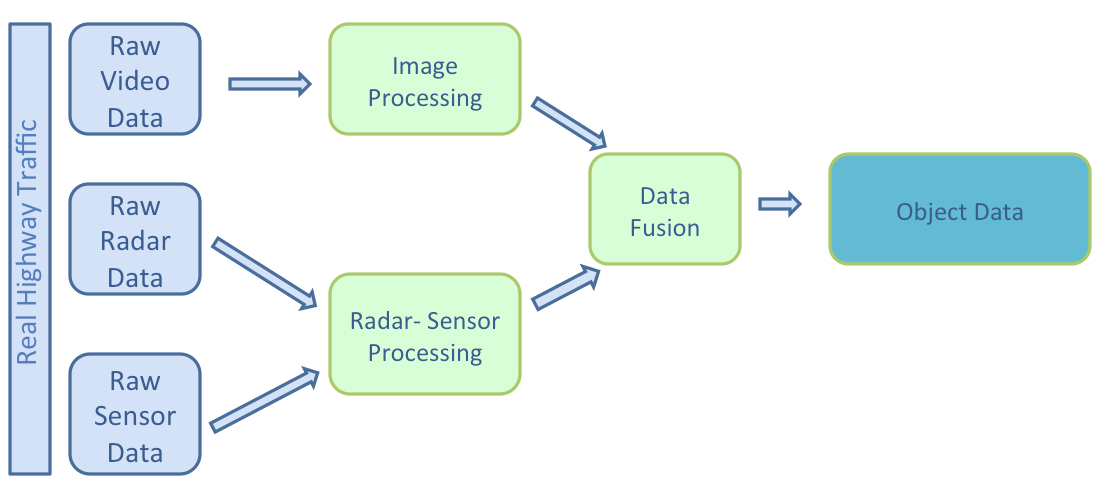
\includegraphics[scale=0.35]{./figures/DaimlerDataFlow}
\caption{\label{Figure:DaimlerDataFlow} Daimler's Data Flow.}
\end{center}
\end{figure}

As can be seen in the above figure, in a first step the raw data coming for the the video, radar and sensors is preprocessed. In a second step this preprocessed data is fused and the high-level or ``object data'' describing the traffic scene is obtained. 

Using this ``object data'', Daimler has developed a probabilistic graphical model [] which is able to recognize an ongoing maneuver around 0.6 seconds before the maneuver really takes place. This probabilistic approach is based on modelling the problem in different layers as shown in Figure \ref{Figure:DaimlerHierarchicalModelling}.


\begin{figure}
\begin{center}
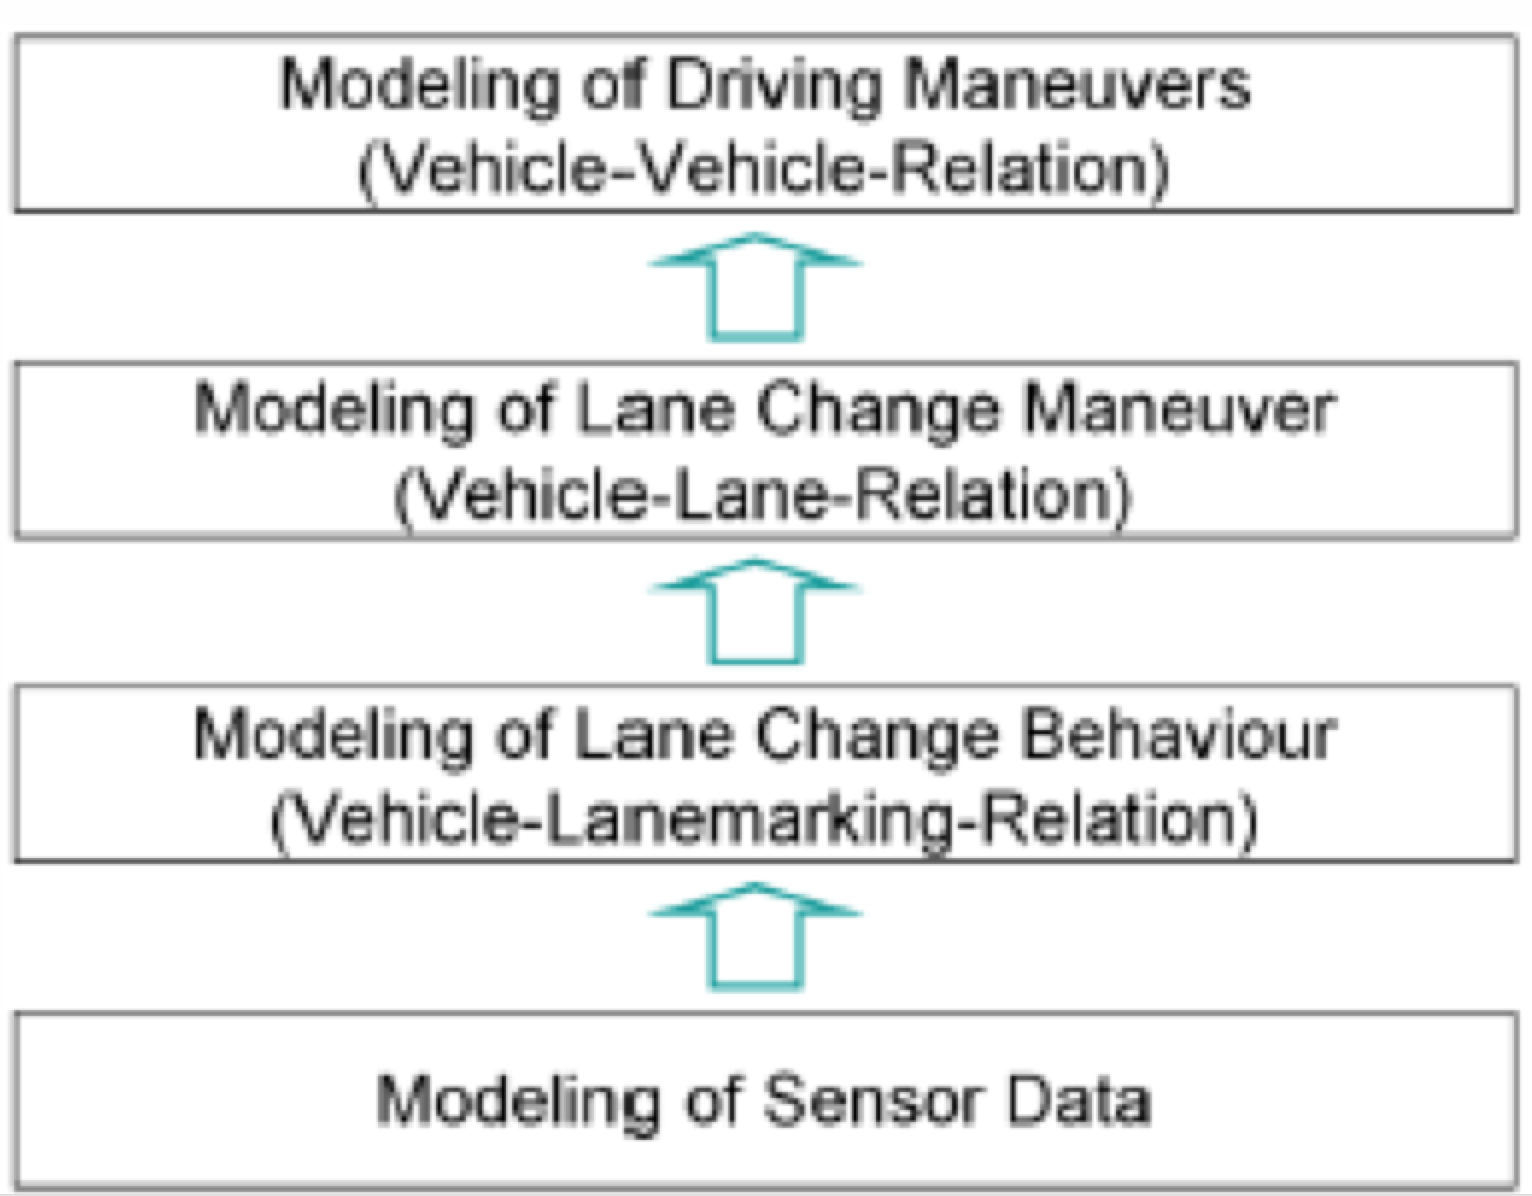
\includegraphics[scale=0.35]{./figures/DaimlerHierarchicalModelling}
\caption{\label{Figure:DaimlerHierarchicalModelling} Static-OOBN model for the prediction of an event (maneuver).}
\end{center}
\end{figure}

In a first step the sensor data is modelled and, sequentially,  a new layer is created on top of that to detect a lane change behaviour. Understanding the lane change behaviour of the vehicles, the system is able to model the lane change maneuver. And, with this information, the system is able to decide the kind of driving maneuver is taking place between pair of vehicles. 



\subsubsection*{The static-OOBN model}

As commented above, this model will work with ``object data''. This data mainly consists on a set of measured and/or computed signals or situation features denoted by $S$ (i.e. EGO speed, EGO lateral velocity, speed of a car in-front, etc.)  describing the traffic scene. 

The causal probabilistic treatment of these signals or situation features allows exploiting heterogeneous sources of information and the quantitative incorporation of uncertainties in the measured signals. The general structure of the static-OOBN model consists of a number of abstraction levels (see Figure \ref{Figure:DaimlerOOBNAbstraction}): all measured and/or computed signals $S$ are handled with their uncertainties $\sigma^2$. These are represented as object classes at the lowest level (class $S$) of the OOBN. The real values $\mu$ of evidence signals are then used at the next level of hierarchy to evaluate the hypotheses (class $H$ in Figure \ref{Figure:DaimlerOOBNAbstraction}). The combined evaluation of several hypotheses results in the prediction of events, class E. In our case: the events are modelling traffic maneuvers of the own and neighbour vehicles.

\begin{figure}
\begin{center}
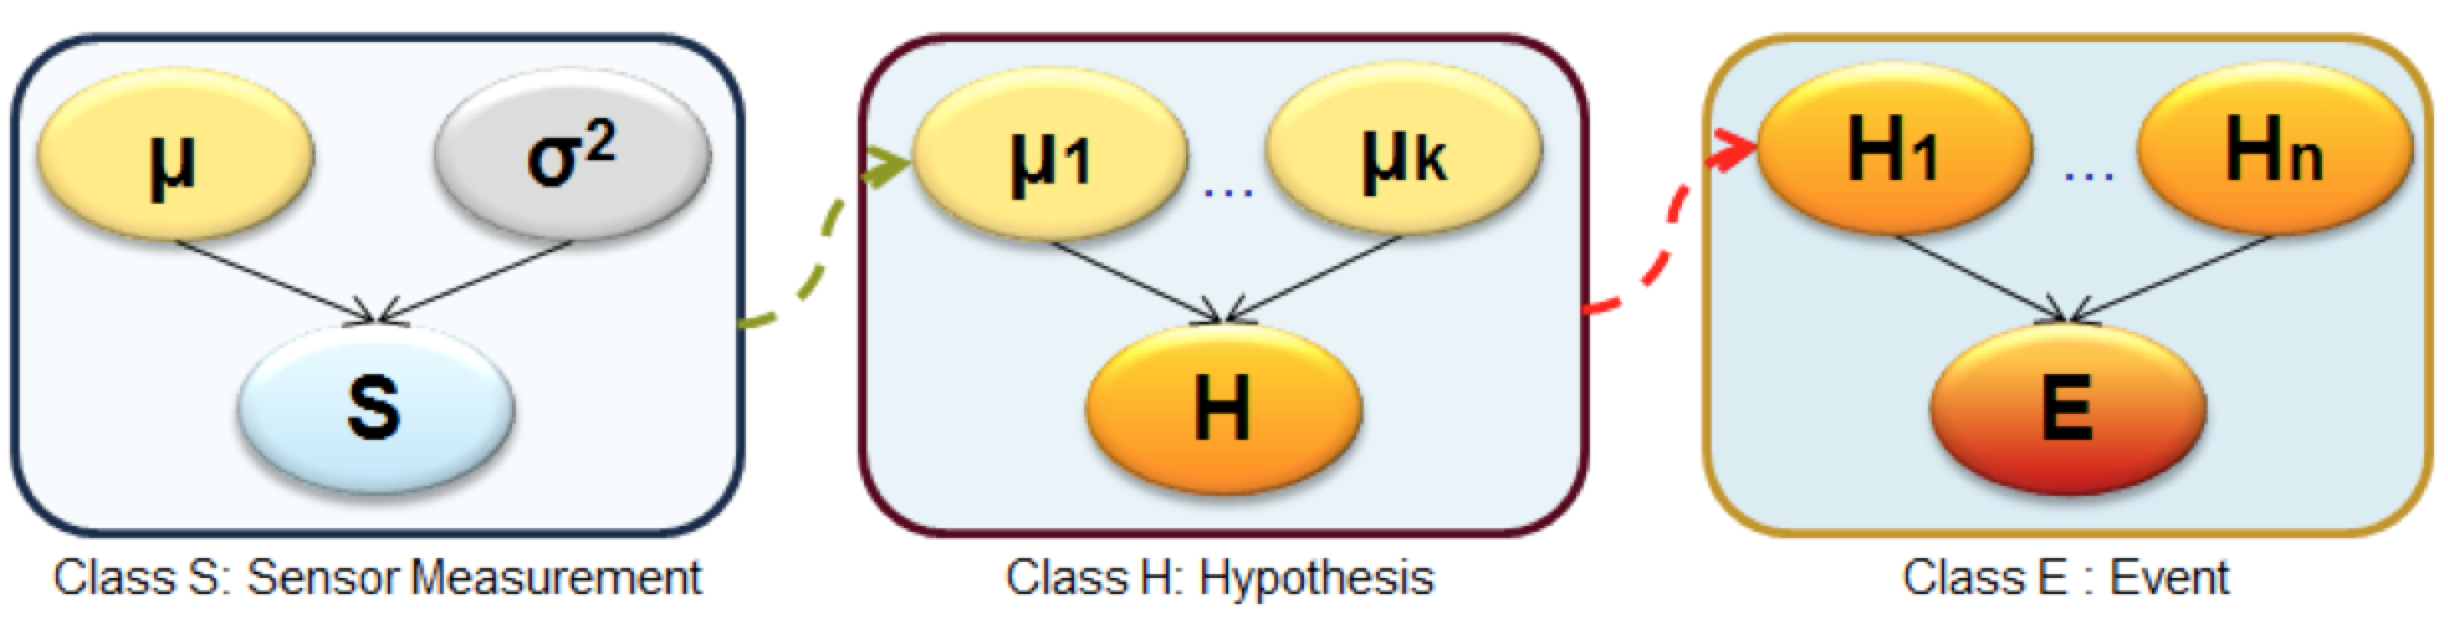
\includegraphics[scale=0.35]{./figures/DaimlerOOBNAbstraction}
\caption{\label{Figure:DaimlerOOBNAbstraction} Static-OOBN model for the prediction of an event (maneuver).}
\end{center}
\end{figure}

As commented above, the observations characterizing a situation are acquired from sensors and computations and, in consequence, are \textit{measured data}. If the measurement instrument is not functioning properly (due to sensor noise or fault), then the sensor-reading ($S\_MEASURED$) and the real variable ($S\_REAL$) under measurement need not to be the same. This fact imposes the causal model structure as shown in Figure \ref{Figure:DaimlerSensorModelling}. The sensor-reading of any measured variable is conditionally dependent on random changes in two variables: real value under measurement ($S\_REAL$) and sensor fault ($S\_SIGMA$).

\begin{figure}
\begin{center}
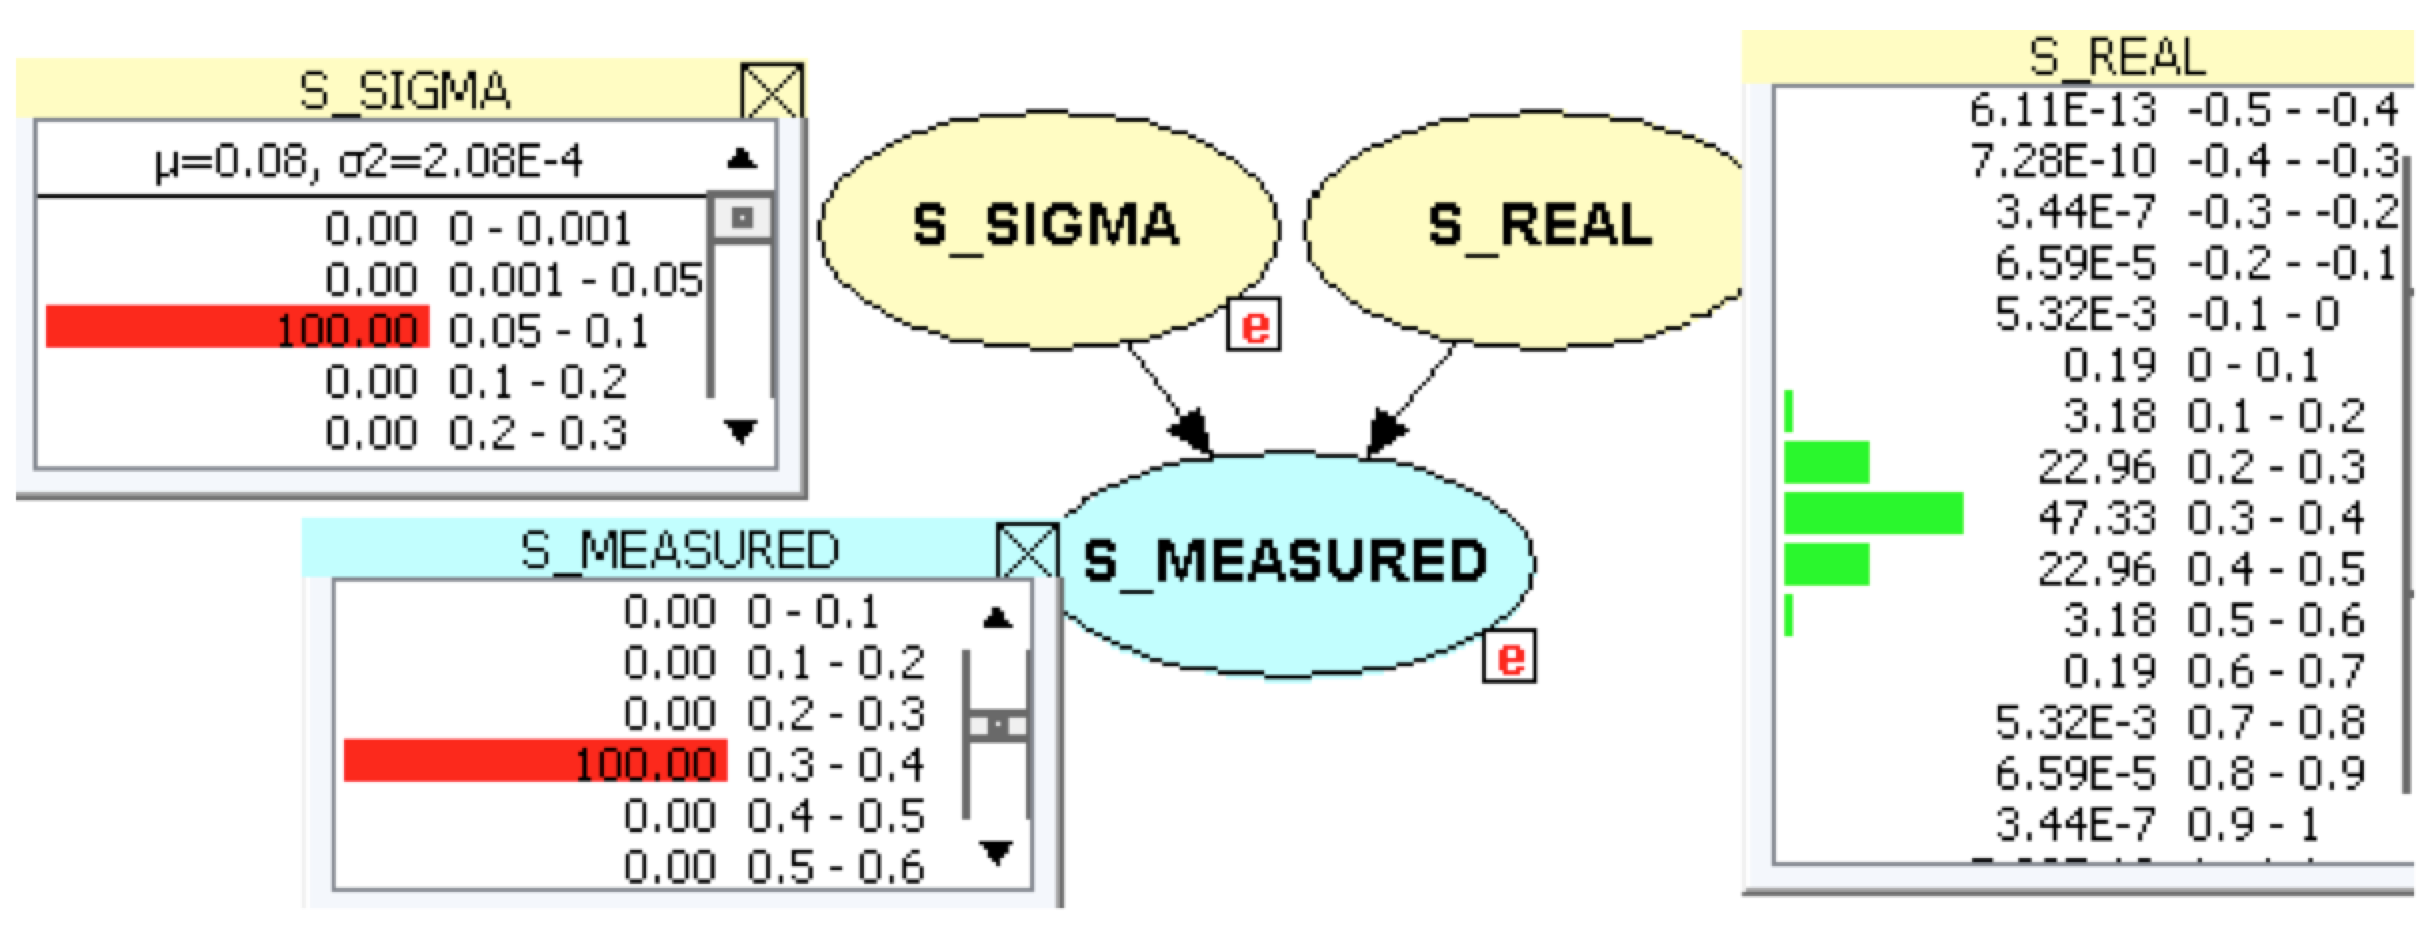
\includegraphics[scale=0.35]{./figures/DaimlerSensorModelling}
\caption{\label{Figure:DaimlerSensorModelling} BN fragment for modeling of sensor’s uncertainties with a discrete ``measurement'' variable.}
\end{center}
\end{figure}


The situation features used for maneuver recognition are structured along three main dimensions: lateral evidence (LE), trajectory (TRAJ), and occupancy schedule grid (OCCGRID). They represent the three hypotheses (see Figure \ref{Figure:DaimlerOOBNAbstraction}), which are modelled by the corresponding OOBN-fragments. For more details see [13], [14]. The hypothesis LE is shown in Figure \ref{Figure:DaimlerLE}. Its conditional probability distribution is represented by a sigmoid (logistic) function to expresses the growing probability for the lateral evidence on crossing the lane marking, when the vehicle is coming closer to the lane marking (modeled by $O\_LAT\_MEASURED$) by growing lateral velocity (modeled by $V\_LAT\_ MEASURED$).

\begin{figure}
\begin{center}
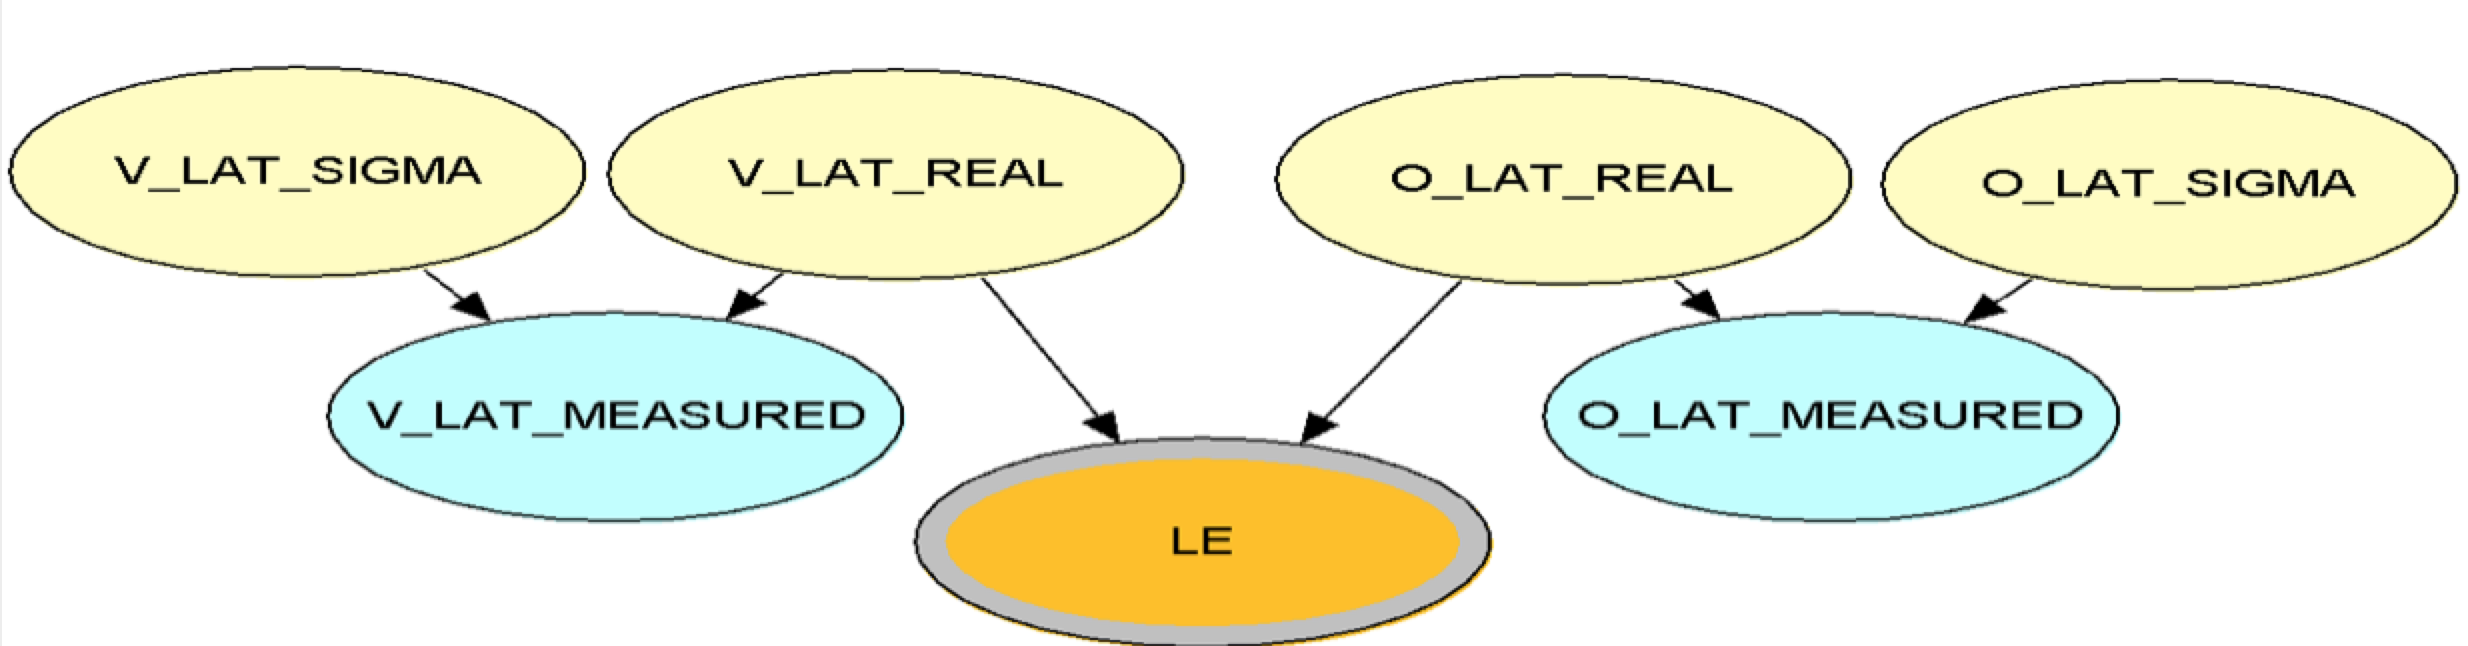
\includegraphics[scale=0.35]{./figures/DaimlerLE}
\caption{\label{Figure:DaimlerLE} BN fragment for modeling of sensor’s uncertainties with a discrete ``measurement'' variable.}
\end{center}
\end{figure}

Figure \ref{Figure:DaimlerOOBNAbstraction} abstractly shows how these hypotheses are combined into events, which in our automotive scenario correspond to the different driving maneuvers: lane follow, lane change (cut-in, cut-out), expressed for ego and surrounding objects, see [12], [13].


\subsubsection*{The dynamic-OOBN model}

